\documentclass{instructions}

\usepackage{xspace}

\newcommand{\git}{\texttt{git}\xspace}
\newcommand\bs{\char`\\}

\title{git: The basics}
\date{\today}

\summary{
This tutorial aims at giving you a good overview of the basics of \git. Steps will
be provided both for the command-line (Linux, MacOSX users) and the graphical
``GitHub for Desktop'' application (MacOSX, Windows users). Even if you use the graphical user
interface, we recommend you to carefully read the equivalent command line
instruction to understand what happen ``behind the scene''.

}

\objectives{
To be able to create a code repository, to understand and be able to create
commits, to be able to share code amongst a group of people using GitHub's
\emph{pull requests}.
}

\begin{document}

\maketitle

\intro

If you have not yet installed \git on your system, here the brief
summary:

\git installation depends on your operating system. If running Linux,
everything is simple, just install \git with your distribution's
favorite package manager (on Debian/Ubuntu,
\texttt{sudo apt-get install git}).

On Windows/MacOSX, we recommend you to use the GitHub official app, that takes
care of properly configuring \git for your system, and also provide an
easy to use user interface (but obviously, an ``easy to use'' interface also means
that it hides things from your eyes, and makes the underlying mecanisms harder to
understand. Anyway...) Head to \url{https://desktop.github.com/}

\note{
Once installed, the Windows GitHub app also provides a link to the Windows
shell, conveniently configured to work with Git. We encourage you to make use of
it and use the command-line based instructions below.  }

While not necessary to use \git, we will make use of GitHub today: if you do not
already have an account, create one, either from the desktop application, or
from the website.

\part{A first git repository}

\step{Initial configuration}

If this is the first time you are using \git, you need to tell it what is your
name and what is your email address, so that all your code contribution are
effectively attributed to you.

From the command-line, type:


\begin{shcode}
$ git config --global user.name "Surname Lastname"
$ git config --global user.email "<email>"
\end{shcode}

If using the GUI, the app will ask you for these details on the first run.

\step{Create a new local repository}

Simply create a new directory (like \url{/home/<username>/src/first-git-repo}) and initialize
it by typing \texttt{git init} from within the directory. The name of this
directory becomes the name of your repository.

If you are using the GUI, click on the big ``plus'' button and create a new repo,
for instance here:\\
\texttt{C:\bs{}Users\bs{}<username>\bs{}Documents\bs{}src\bs{}first-git-repo}

That's it: a \git \textbf{repository} is simply a regular directory, with one
special item: an hidden \texttt{.git/} directory that stores all the
\textbf{objects} \git manipulates (mainly binary blobs representing files or
parts of files).

\step{A first commit}

One of the first steps after creating a new repository is to add a
\texttt{README} file that describes briefly the content of the repository:
create such a file and describe in 2-3 lines the new CoolApp\copyright you are going to
develop.

\more{It's nowadays common practise to write \texttt{README}s using the \textsc{markdown} syntax
    (extension \texttt{.md}): \textsc{markdown} is a markup language that lets you write simple text
    documents that are structured and can be nicely rendered by the computer.

    Learn more about \textsc{markdown} on Wikipedia:
    \url{http://en.wikipedia.org/wiki/Markdown}
}

Then, \textbf{commit} this \textbf{change}: since the file \texttt{README} is
not yet known to \git, first \textbf{add it}: \sh{git add README}, and
then create a new \textbf{commit} with \sh{git commit}. If using the GUI, simply
make sure the file is checked in the \emph{Changes} tab of the GUI.

\git will ask you for a
commit message (a commit message is made of a mandatory one-line \emph{summary} --
usually maximum 72 characters long -- and a longer, optional, \emph{description} that explains
in greater details what this commit is about).

The commit summary must be concise yet must describe accurately the content of
the change. For now, use the simple commit message ``Added a README''.

\note{
    You can use \sh{git commit -m"commit message"} to directly create a commit
    with a commit message.
}

By typing \sh{git log} (or just looking at the \emph{History} tab of the GitHub GUI), you can see the
history of changes in your repo. On Linux, \texttt{gitk} is another
convenient way to display in a graphical way the history of the repo.

\step{Code versioning}

Download this nice embryo of a TicTacToe game:\\
\url{https://raw.githubusercontent.com/severin-lemaignan/git-presentation/master/sample-code/main.cpp}

Add it to the \git repository. Commit this change.

Now, change the coordinates of the TicTacToe grid to use the numerical
coordinates \texttt{1, 2, 3} instead of \texttt{A, B, C}, as it simplifies the code.

Using \sh{git status} or the GUI, review the change and commit it (\sh{git
commit <your file>}, choosing an appropriate commit message.

\part{Going social}

Until now, you have only worked on a \textbf{local} \git repository: this is a
perfectly legitimate use of \git. As a \textbf{distributed version control
system} (DVCS), \git is meant to support a wide range of code workflows,
including purely local workflows: if you do not need to share your code over
Internet, why would you need an Internet connection to benefit code versioning?

However, \git is particularly powerful when working in groups: the core idea is
that each participant own a full copy of a repository, and exchanges commits
through \textbf{pushes} (to send commits to others) and \textbf{pulls} (to get
commits from others). As you can see on the figure below (and contrary to
traditional VCS like SVN), you \textbf{do not
need to use a central server} (but you can!): \git is distributed, each
participant own a full, autonomous copy of the repository and can obtain
(\emph{pull}) commits from any other participant.

\begin{center}
    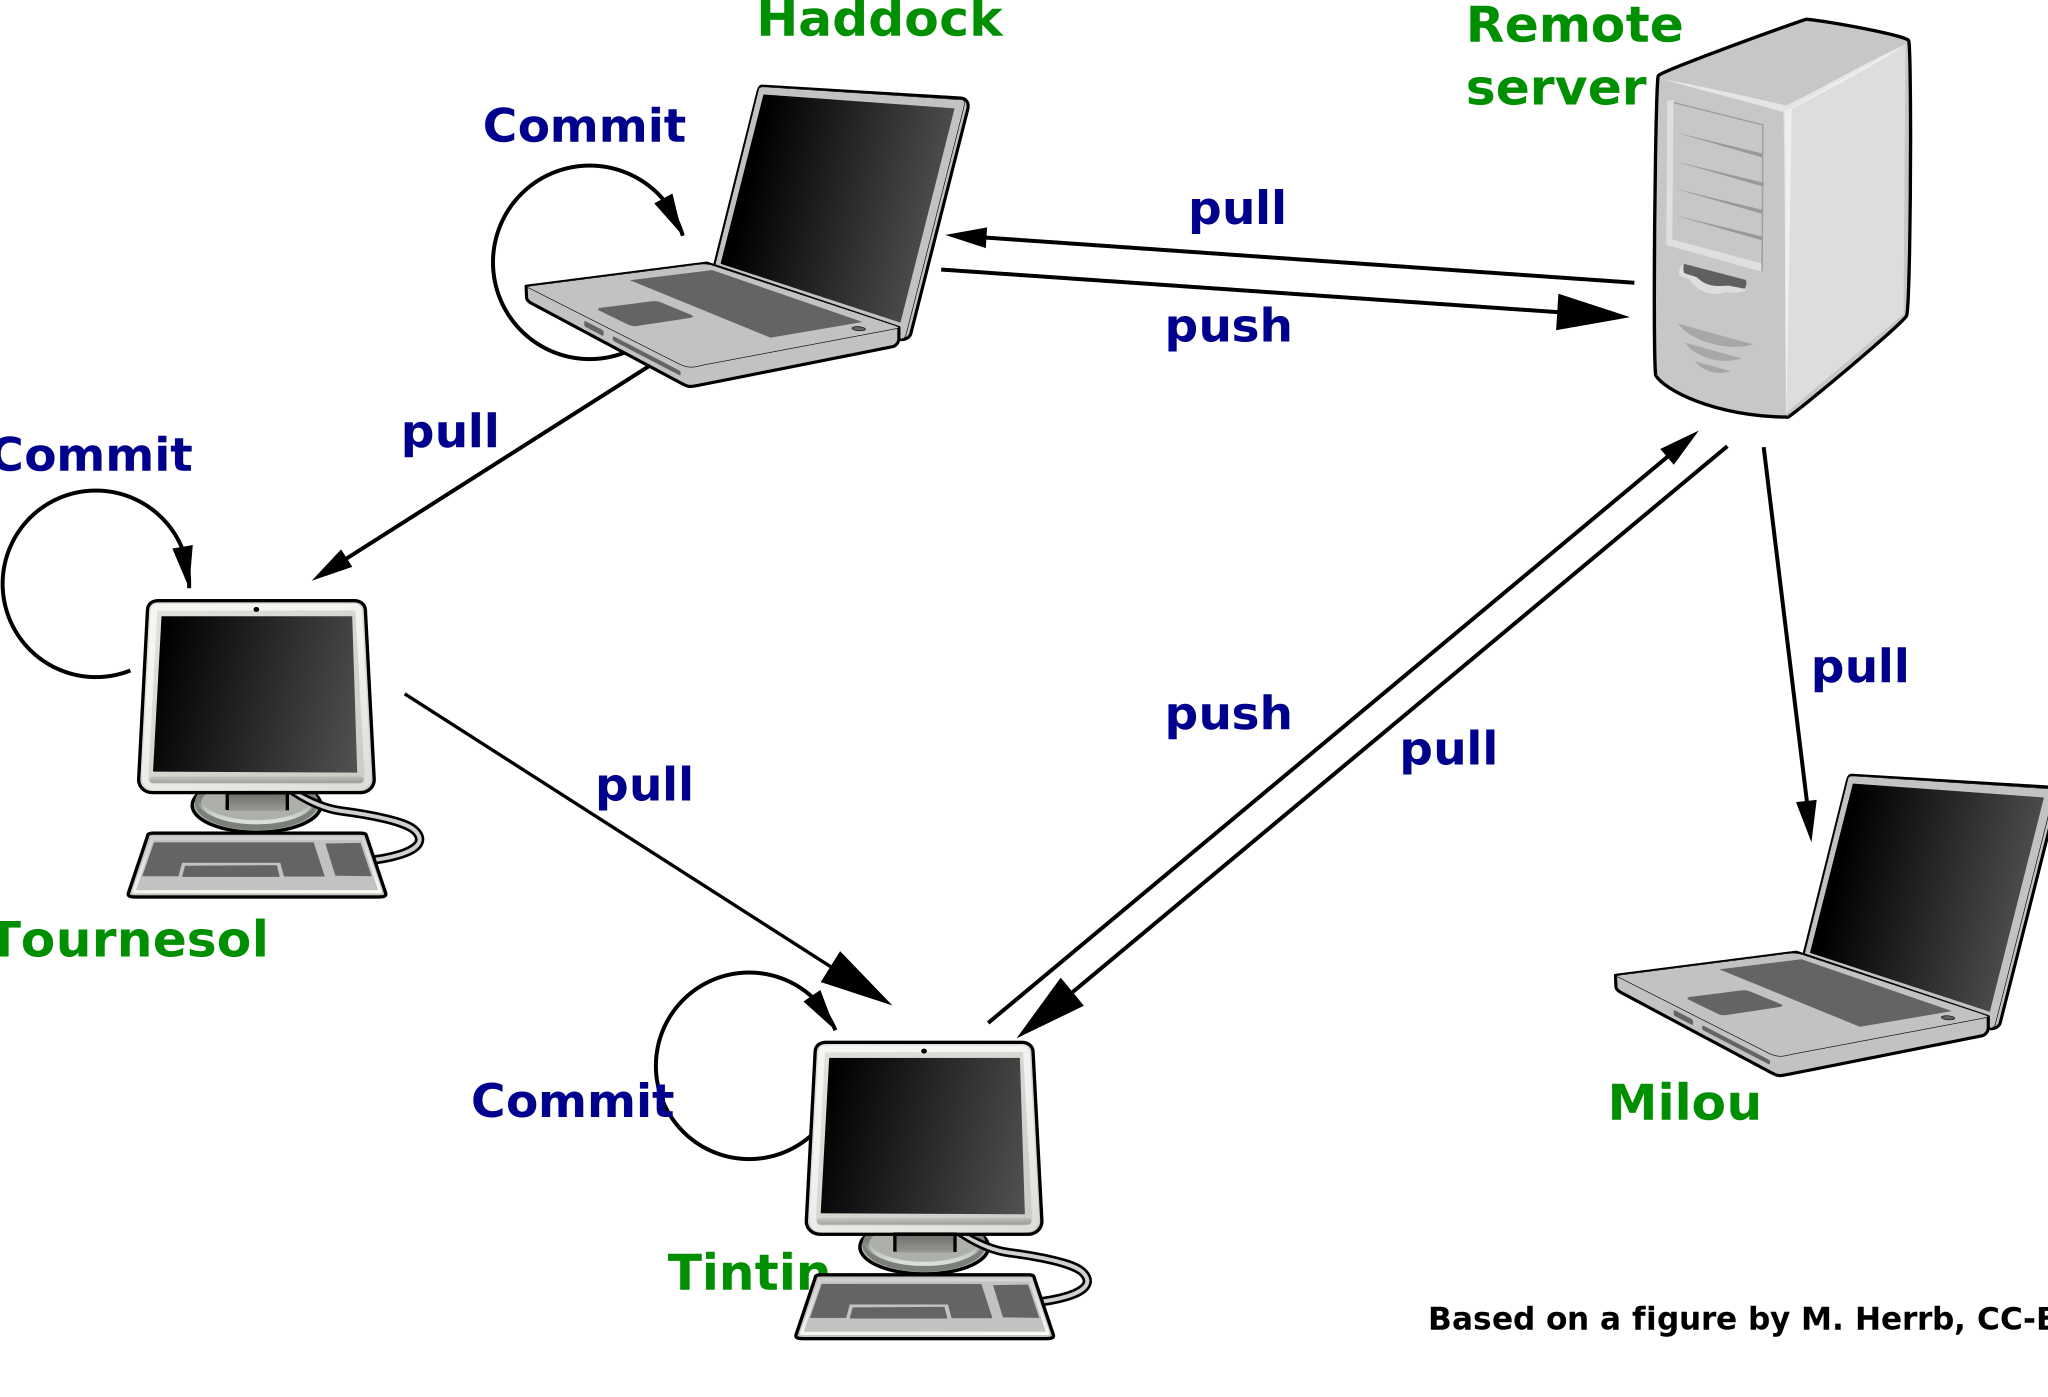
\includegraphics[width=0.8\linewidth]{figs/distributed-git.pdf}
\end{center}

Distant repositories can be on a remote Internet server like GitHub, on your
colleagues' computers,
or even on a USB stick that you carry over with you. \git calls them
\textbf{remotes}. You can add as many remotes as you want to your local
repository by giving them names.

Often, you will have one main remote, which is traditionally called
\texttt{origin} (but it's up to you to choose a different name!).

\step{Adding a remote}

You will add GitHub as a remote repository to your local \git repository (feel
free to adapt the instructions if you are using another remote like
\url{git.epfl.ch}).

First create an empty repository on GitHub:

\begin{center}
    
\includegraphics[width=0.3\linewidth]{figs/github-new.png}
\end{center}

Name it after your local repository (not mandatory, but convenient), and do
\textbf{not} check the checkbox ``Initialize this repository with a README''
since you already have one.

Then, add this remote to your local repository, and \textbf{push} your changes
online:

\begin{shcode}
$ cd <REPO DIR> # for instance $HOME/src/first-git-repo
$ git remote add origin https://github.com/<account>/<repo>.git # add a remote called origin
$ git push -u origin # push all your local commits to GitHub
\end{shcode}

\note{
    If you are using the GitHub GUI, adding a \underline{GitHub} remote is easy:
    just press the \emph{Publish} button: the GitHub app while create
    a new remote repository for you and immediately push the changes.
    
    However, if you want to use a non-GitHub remote, you need to use the command
    \sh{git remote add...} to setup the remote. You can then use the GUI
    normally, also with this new remote.
}

\more{
    In this example, you use the \texttt{https} protocol as \textbf{transport}
    between the remote server and your local repository. This requires you to
    type you login and password every time (this is not really an issue when
    using the GitHub app since it remembers your credentials).
    
    \git is however often used with \texttt{ssh} as transport. No password is
    required in that case (it transparently uses your \texttt{ssh} keys to establish
    an encrypted connection to the remote server). You can easily configure
    your GitHub account to use \texttt{ssh}. Read the documentation here:\\
    \url{https://help.github.com/articles/generating-ssh-keys/}
}

\step{Explore the GitHub web interface}

Go to the GitHub website, log in, and navigate into your repository to check that
your \texttt{README} file is indeed there.

Besides hosting your code, GitHub allows you to also create \textbf{Issues} to
track what need to be done or corrected in your project. Go to the \emph{Issues}
panel
$\vcenter{\hbox{
\includegraphics[scale=0.8]{figs/github-issues-icon.png}}}$ and
create a new issue (for instance, to suggest to use deep learning to implement
the TicTacToe AI). \textbf{Label} the issue as a
proposed \emph{Enhancement}.

Note the issue number that GitHub displays after the title of the issue (or in the address
bar), probably \texttt{\#1} since this is the first issue you are reporting. You
will make use of this number soon.

\step{Propose a code contribution}

You will now team with your neighbour to propose a fix for the issue he/she has
opened in his/her project.

To this end, you need to go through three steps, detailed below:
\begin{enumerate}
    \item \textbf{clone} his/her repository to get a local copy of his/her
        repository,
    \item improve his/her code and commit the resulting change,
    \item propose him/her to \textbf{pull} your change
\end{enumerate}

(1) requires you to retrieve the \textbf{clone URL} of your teammate
repository by going to his/her GitHub page and looking down on the right column:

\begin{center}
    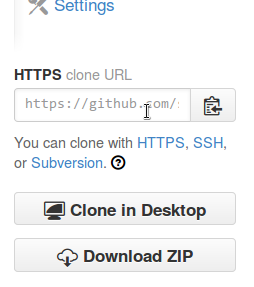
\includegraphics[width=0.3\linewidth]{figs/github-clone.png}
\end{center}

\note{The \emph{Clone in Desktop} button only appears on Windows and MacOSX and
opens the GitHub application to clone the repository from the app.}

Copy the URL, and then:

\begin{shcode}
$ cd <SOURCE DIR> # for instance $HOME/src
# Clone the repo <repo> inside directory <dir_name> (same as <repo> if omitted)
# To avoid confusion with your own repository, use smthg like 'first-git-repo-gerard' as dir_name
$ git clone https://github.com/<account>/<repo>.git <dir_name>
\end{shcode}

You now have a full copy of the repository on your local machine in
\texttt{<dir\_name>}. Edit the source of your teammate to (attempt to) correct the
the issue he/she opened, and commit the result.
In this case, a good commit message would be: ``Fixing <description of issue> (issue
\#1)''. By referencing the GitHub issue number in the commit message, GitHub will
automatically link your commit to the issue.

Several options are available to send your changes to your teammate, including
pushing them to your teammate's repository (if you are allowed to do so!),
sending them as a patch over email, making the directory of your local repo
available from the web so that the other one can \emph{pull} your changes,
exporting your changes as a patch file that can be shared via an USB key, etc.

However, a common and convenient way to propose code relies on sending a
\textbf{pull request} to the teammate via GitHub.

To do so, we need to go through the following four steps, that are detailed
below:

\begin{enumerate}
    \item create a new repository on your GitHub account by \textbf{forking} the
        original repository (what GitHub calls a fork is simply a copy of an
        existing GitHub repository to your own account),
    \item add this repository as a second remote to your local repository,
    \item push the changes to this remote,
    \item create a pull request from GitHub's web interface.
\end{enumerate}

\note{
    Items (1) and (2) are only required the first time.
}

(1) is achieved by navigating to the original project's GitHub page and
clicking on the \emph{Fork} button:

\begin{center}
    
\includegraphics[width=0.35\linewidth]{figs/github-fork.png}
\end{center}

\note{
    If you have a repository named identically to the repository that you are
    forking, GitHub will rename it like \texttt{<repo\_name>-1}. You can change
    this name from the GitHub web interface, in the \emph{Settings} menu (last
    icon in the right column).
}

You already know how to perform the second step. Since \texttt{origin} is
already the name of your teammate's remote repository, make sure to give this
remote a different name (for instance \texttt{myfork}).

\note{\texttt{git remote -v} lists the existing remotes with their URLs.}

\note{For GUI users: the GitHub application does \underline{not} support several
    remotes. You can either use the shell to add a second remote as explained
    above, or simply set your fork as the default remote (\texttt{origin}):
    within the GitHub application, select the repository of your teammate, then
    click on the small gear in top right corner and select \emph{Repository
    settings...}. Replace the URL of the \emph{Primary remote} by the URL of the
    repository on your own GitHub account.
}

You can then push your changes to the remote hosted on your own GitHub account:
\sh{git push myfork} (or click on the \emph{Sync} button in the GitHub GUI).

You can now create and submit a pull request: go to your GitHub account on the
web. GitHub offers you to create a pull-request:

\begin{center}
    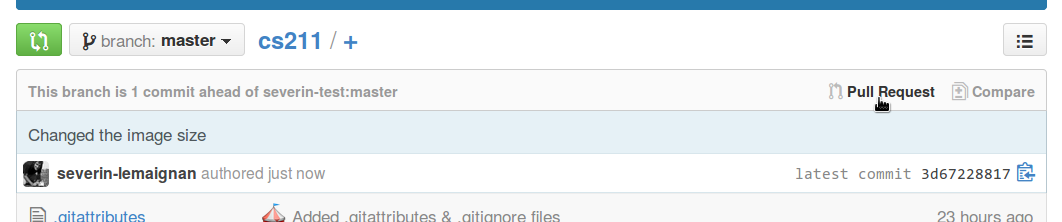
\includegraphics[width=0.8\linewidth]{figs/github-pr1.png}
\end{center}

Click the link. GitHub lets you select where you want to send the pull request
(the \emph{base fork}, by default the repository that you initially forked), and
you can review the changes that will be included.


\begin{center}
    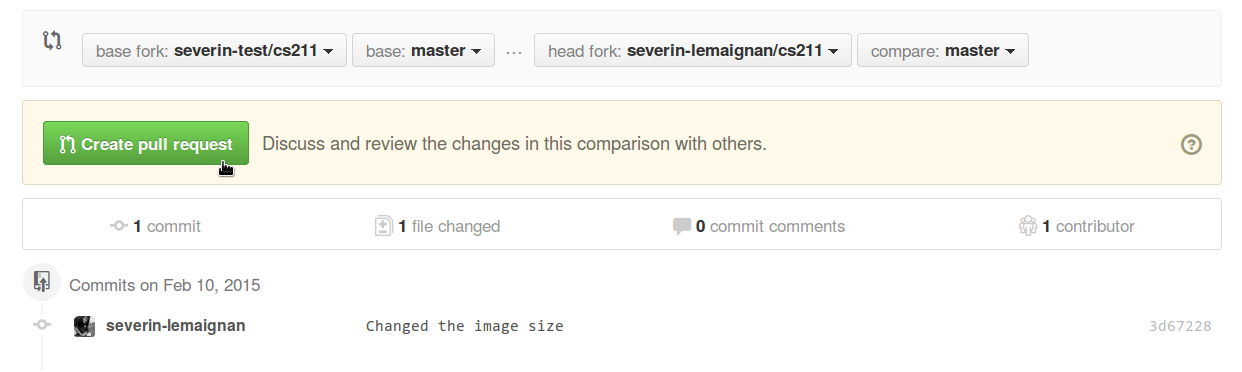
\includegraphics[width=0.8\linewidth]{figs/github-pr2.png}
\end{center}

Create and send the pull request.

\step{Review, discuss and merge a pull request}

You have sent a pull request to your teammate, and he/she did the same: you
should now review your partner's contribution.

Navigate to your initial repository, and display the list of pending pull
requests ($\vcenter{\hbox{
\includegraphics[scale=0.8]{figs/github-pr-icon.png}}}$ button).

Select the open pull request, click on the commit(s) to review the changes, use the
comment box to discuss the change (or to simply say ``Thank you!'' if everything
looks good), and finally \textbf{merge} the pull request:

\begin{center}
    
\includegraphics[width=0.8\linewidth]{figs/github-merge-pr.png}
\end{center}

To retrieve these changes in your local repository, simply run \sh{git pull} (or
press the \emph{Sync} button) from your local repository (\texttt{first-git-repo}).

\more{
    If you think the pull request needs further refinement, explain in the
    comment box what is missing for this change to be merged (errors, style,
    undesirable feature...). The author of the pull request can then
    \textbf{update} his/her pull request by adding (or modifying) commits and
    pushing them again to his/her fork. The pull request will be
\textbf{automatically updated}, no need to create a new pull request.
}

%\part{Working with branches}
%
%
%
%\begin{shcode}
%# define a few colors
%RED='\[\e[0;31m\]'
%GREEN='\[\e[1;32m\]'
%CYAN='\[\e[0;36m\]'
%WHITE='\[\e[1;37m\]'
%NC='\[\e[0m\]'  # No Color
%
%function get_git_branch {
%    git branch --no-color 2> /dev/null | sed -e '/^[^*]/d' -e 's/*\(.*\)/\ \[\1\]/'
%}
%
%PS1="${WHITE}[${GREEN}\u@\h${WHITE}]${CYAN}\w${RED}\$(get_git_branch)${WHITE} $ ${NC}"
%\end{shcode}
%

%\part{The CS211 project workflow}
%
%
%
%\begin{shcode}
%
%$ cd <WORK DIR> # for instance $HOME
%$ git clone https://github.com/chili-epfl/cs211-visual-computing.git -o epfl
%$ cd cs211-visual-computing
%$ git branch
%* master
%$ git remote add origin https://github.com/<account>/<repo>
%$ git push -u origin
%
%\end{shcode}
%
%\more{\git stores the configuration of the repository (remotes, branches, etc.)
%    in file named \texttt{config}, within the hidden \texttt{<your\_repo>/.git} repository. You
%    can have a look (\sh{cat .git/config}) and even edit it directly (for
%    instance to change a remote name or URL) but be careful not to break
%    anything!
%}
%
%Checkout this week's branch:
%
%\begin{shcode}
%
%$ git checkout -b week1 epfl/week1
%
%\end{shcode}
%

\part{The next steps}

\git is a large system that may appear complex at first sight. Take some time to
get used to it: becoming familiar with \git will be soon rewarding! and do not
hesitate to ask questions during the coming weeks.

This tutorial did not introduce many concepts like \textbf{branches},
\textbf{conflicts} or \textbf{rebase}. If you want to learn more on \git, here a
few resources (besides your lovely teaching assistants!):

\begin{itemize}
    \item Many \git \emph{cheatsheets} exist. Tower has a good one
        (\url{http://www.git-tower.com/blog/git-cheat-sheet/}), GitHub as well
        (\url{https://help.github.com/articles/git-cheatsheet/}, including a
        French version), and a nice
        interactive cheatsheet is there:
        \url{http://ndpsoftware.com/git-cheatsheet.html} (French translation
        also available)
    \item \emph{git from the bottom up} is a great (and esay) reading to understand how
        \git actually work. As a matter of fact, most \git commands become evident once you know how they are
        built. \url{https://jwiegley.github.io/git-from-the-bottom-up/}
\end{itemize}
\end{document}
